\documentclass[bigger]{beamer}

\usepackage[utf8]{inputenc}
\usepackage{booktabs}
\useinnertheme{rounded}
\usecolortheme{crane}
\setbeamerfont{block title}{size={}}

\newcommand{\img}[2]{\begin{center}\includegraphics[width=#1\linewidth]{#2}\end{center}}

\title{Umíme: Data-Driven Techniques for Avoiding Stupidity}

\author{Radek Pelánek\\[10mm]
  
\includegraphics[width=.2\linewidth]{al-logo-researchgroup}}

\date{2022}

\begin{document}

\frame{\titlepage}

\begin{frame}
  \frametitle{Context}

  \begin{itemize}
  \item Umíme \texttt{https://www.umimeto.org/}, research spin-off, Czechia
    (\~ 15\% Czech schools with licence)
  \item small team, wide coverage (math, programming, Czech, English,
    geography, ...)
  \item data-driven techniques for prioritization, focusing attention of
    content developers
  \item ``avoiding stupidity perspective''\\
    \emph{Improving Learning Environments: Avoiding Stupidity Perspective, IEEE
      TLT, 2022}
  \end{itemize}
\end{frame}

\begin{frame}
  \frametitle{Typical Techniques Used}

  \textbf{simple basic techniques}
  \begin{itemize}
  \item success rate
  \item response times
  \item common wrong answers
  \end{itemize}

  \bigskip

  \textbf{thoroughly analyzed}
  \begin{itemize}
  \item multiple visualizations for better interpretation
  \item automatic detection of problematic cases
  \item biases, cheating
  \end{itemize}
\end{frame}

\begin{frame}
  \frametitle{Example}

  word problems, division with remainder

  \img{.9}{wp-division-remainder}

  {\small green = ``easy'' set, blue = ``medium'' set}
\end{frame}

\begin{frame}
  \frametitle{Word Problems: Overview}

  \img{.9}{wp-overview}
\end{frame}

\begin{frame}
  \frametitle{Word Problems: Overview II}

  \img{.9}{wp-overview-2}
\end{frame}

\begin{frame}
  \frametitle{Outlier Detection}

  \img{.9}{wp-mult}
\end{frame}

\begin{frame}
  \frametitle{Ordering of Problems}

  context: interactive problem solving

  \bigskip

  \begin{tabular}{lll}
    point reflection & parallel lines & triangles \\
    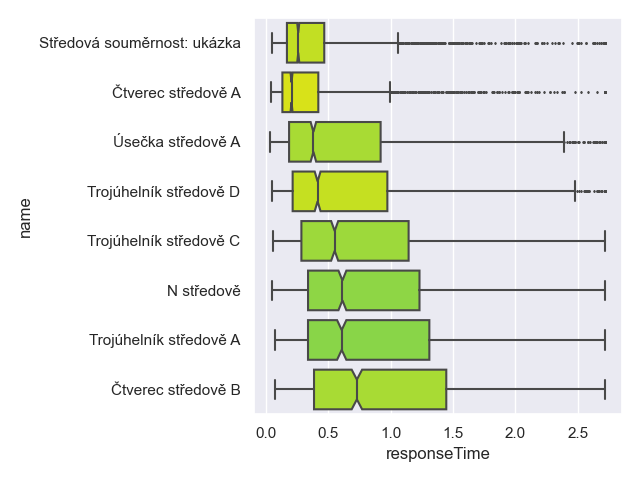
\includegraphics[width=.3\linewidth]{mrizkovana_stred} &
    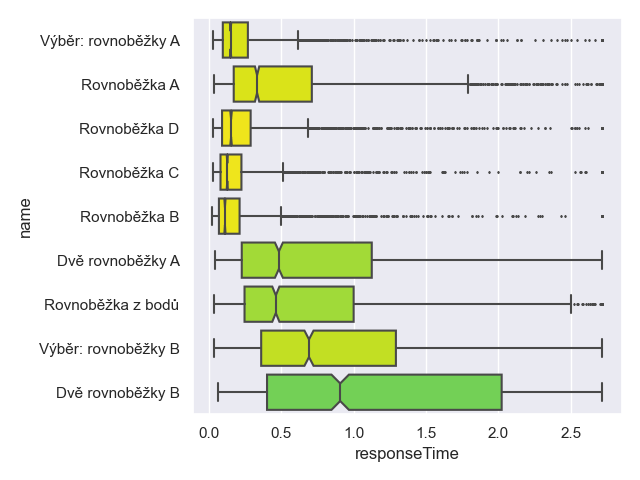
\includegraphics[width=.3\linewidth]{mrizkovana_rovnobezky} &
                                                                  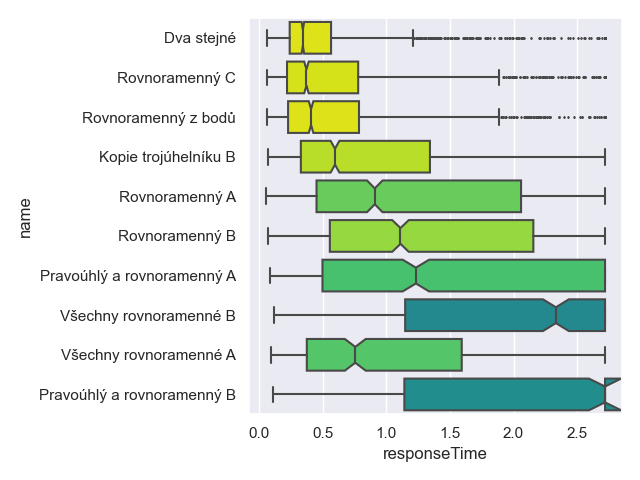
\includegraphics[width=.3\linewidth]{mrizkovana_triangles} \\
    OK & add problems  & reorder, \\
                     & of medium difficulty &  check the two \\
    & & difficult
                                             examples \\
  \end{tabular}
\end{frame}

\begin{frame}
  \frametitle{Common Wrong Answers}

  \img{1}{common-wrong}

  $\Rightarrow$ add more examples of the type $8-(8+t)$
\end{frame}


\begin{frame}
  \frametitle{Cheating}

  normalized response times: logarithm, division by item median

  \bigskip

  \begin{tabular}{cc}
    division with remainder & quadratic equations \\
    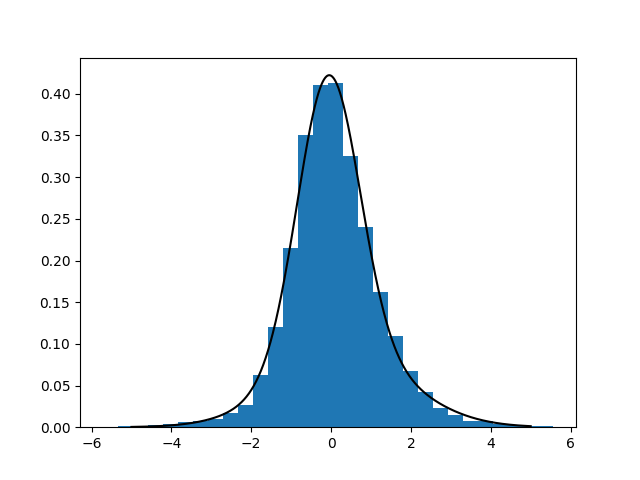
\includegraphics[width=.45\linewidth]{rt-wp-division.png} &
    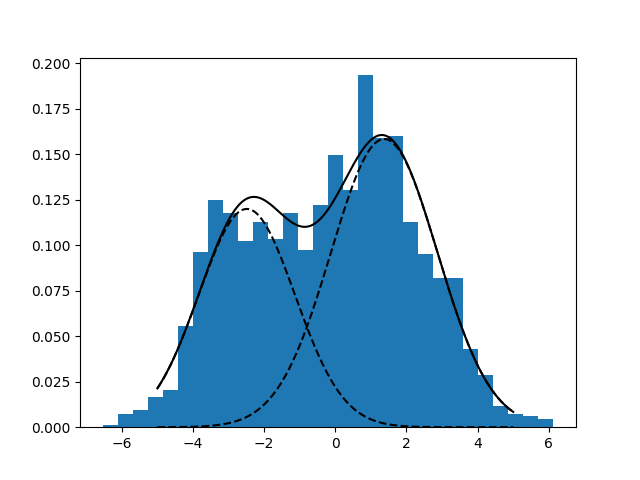
\includegraphics[width=.45\linewidth]{rt-wp-kvadraticke.png} \\
  \end{tabular}
\end{frame}

\begin{frame}
  \frametitle{Summary}

  \begin{itemize}
  \item automated search for problematic content
  \item visualizations for interpretation of data
  \item typical actions:
    \begin{itemize}
    \item add/remove/update items
    \item create scaffolded items and explanations for difficult content
    \item increase granularity of content (split knowledge components)
    \end{itemize}
  \end{itemize}
\end{frame}



\end{document}